\documentclass[11pt]{article}
\usepackage[margin=1.5in]{geometry}
\usepackage{graphicx}
\usepackage{float}
\usepackage{parskip}
\usepackage{amsmath}

\usepackage{pgfplots}
\pgfplotsset{width=10cm, compat=1.9}

\begin{document}

\textbf{\Huge One-Dimensional Motion}

Athan Zhang \& Jeffrey Chen

\section{Displacement}

Physics is the study of the natural world and its interactions. One of the most fundamental and observable phenomena is the idea of movement or motion. The most basic form of this is called \textbf{displacement}, which refers to the change in \textit{position} of an object or point in space. It is definitively represented by a vector quantity as it has magnitude (length of distance traveled) and direction (direction of movement).\footnotemark[1] We use the Greek letter $\Delta$ (uppercase delta) to indicate change in a quantity; thus, the change in position, $x$, is written as $\Delta x$ and is define as:

\begin{equation*}
    \Delta x = x_{2} - x_{1}
\end{equation*}

The metric unit used for displacement is meters (m).

\subsubsection*{Distinguishing from Distance}

It's important to understand the difference between displacement and distance. While commonly understood as the same thing, there are minute displacements. Distance is the quantity of displacement, e.g. it is the magnitude of the displacement vector. It can never be negative and it has no direction, it is only a \textit{value}. Displacement is a vector, distance is a scalar.

\section{Velocity and Speed}

While displacement was a measure of the change of position, \textbf{velocity} measures that change of position \textit{over time}. This means that velocity is a vector  quantity, similar to displacement, that describes the rate at which an object changes its position.\footnotemark[1]

\subsection{Average Velocity}

Average velocity is as its name describes. It measures the change of position from two given points in time. It is define as the ratio of displacement $\Delta x$ to the time interval $\Delta t$:

\begin{equation*}
    v_{avg} = \frac{\Delta x}{\Delta t} = \frac{x_{2} - x_{1}}{t_{2} - t_{1}}
\end{equation*}

The metric unit of velocity is meters per second (m/s). 

\footnotetext[1]{Keep in mind that since both displacement and velocity are vectors, they may be positive or negative. This is simply relative to the axis or frame in which the motion occurs. For example, positive displacement only means movement along the positive direction of the axis established in the frame of reference.}

\subsection{Average Speed}

Average speed is simply the ratio of the total \textit{distance} $\Delta d$ traveled to the time interval $\Delta t$.

\begin{equation*}
    s_{avg} = \frac{\Delta d}{\Delta t} = \frac{|x_{2} - x_{1}|}{t_{2} - t_{1}}
\end{equation*}

\subsection{Instantaneous Velocity}

Unlike average velocity, which is calculated between two points in time, instantaneous velocity defines the velocity of a particle at a \textit{single} instant. We can take the definition of average velocity, and apply a limit to it such that the difference between the two points in time is zero, essentially meaning the two points in time are the same.

\begin{align*}
    v(t) = \lim_{\Delta t \to 0} \frac{\Delta x}{\Delta t} = \frac{dx}{dt}
\end{align*}

This calculation is also the same as calculating the slope of the line tangent to the $x$-versus-$t$ curve at the given $t$. 

The graph below shows a comparison of average and instantaneous velocities. As we calculate the velocity from $t = 2$ to $t = 8,6,4,2$ we see that the slope of the secant or tangent lines, which is the velocity, changes. The ultimate tangent line of the curve at $t = 2$ is the instantaneous velocity.

\begin{center}
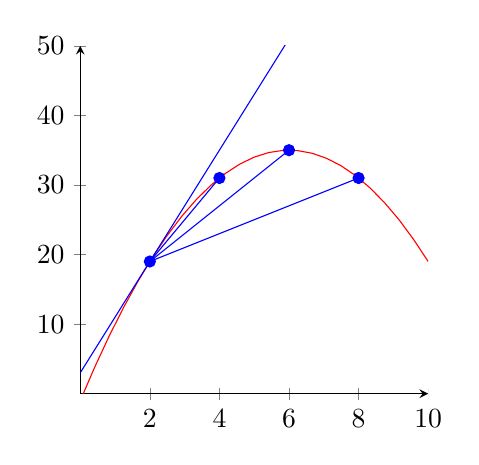
\begin{tikzpicture}
    \begin{axis}[
        axis lines=middle, 
        width=6cm, 
        height=6cm, 
        ymin=0, 
        ymax=50, 
        ytick={10, 20, 30, 40, 50}, 
        xmin=0, 
        xmax=10, 
        xtick={0, 2, 4, 6, 8, 10},
    ]
    \pgfplotsset{dot/.style={color=blue,fill=blue,only marks,mark=*}}
    \addplot[domain=0:10, color=red]{-(x-6)^2 + 35};
    \addplot[domain=0:10, color=blue]{8*x + 3};
    \addplot[domain=2:4, color=blue] {(19-31)/(2-4) * (x-2) + 19};
    \addplot[domain=2:6, color=blue] {(19-35)/(2-6) * (x-2) + 19};
    \addplot[domain=2:8, color=blue] {(19-31)/(2-8) * (x-2) + 19};
    \addplot[dot] coordinates{(2,19)};
    \addplot[dot] coordinates{(4,31)};
    \addplot[dot] coordinates{(6,35)};
    \addplot[dot] coordinates{(8,31)};
    \end{axis}
\end{tikzpicture}
\end{center}

\section{Acceleration}

\textbf{Acceleration} is the rate of change of the instantaneous velocity. The average acceleration for a particular time interval $\Delta t$ is defined as the ratio $\Delta v / \Delta t$:

\begin{align*}
    a_{avg} = \frac{\Delta v}{\Delta t}
\end{align*}

However, just like velocity, we can calculate the instantaneous acceleration at a single instant:

\begin{align*}
    a(t) = \lim_{\Delta t \to 0}\frac{\Delta v}{\Delta t} = \frac{dv}{dt} = \frac{d^{2}x}{dt^{2}}
\end{align*}

We can see that acceleration is simply the second derivative of displacement, which can be rewritten as $\ddot{x}$. A dot above a variable is defined as an order derivative of the variable, thus, the first derivative of displacement $x$ is $\dot{x}$ which is velocity, the second derivative is $\ddot{x}$ which is acceleration, and the third derivative is $\dddot{x}$ which is known as jerk (but less commonly used in physics).

The metric unit of acceleration is meters per second squared (m/s$^{2}$).


\section{Constant Acceleration Equations (CAKE)}

The motion of a particle with a constant acceleration is common in nature. A classic example is the motion of a particle as it falls through space. It is subject to the force of gravity by the Earth, which is constant and measures in at $g = 9.81$  m/s$^{2}$. This is true under the assumption that forces exerted on the particle by air resistance, electromagnetism, or other gravitational pulls, are negligible. 

\subsection{First Kinematic Equation}

If a particle has a constant acceleration $a$, it follows that the average acceleration for any time interval is also $a$. This means that

\begin{align*}
    a = a_{avg} = \frac{\Delta v}{\Delta t}
\end{align*}

Then, if the velocity is $v_{0}$ at $t = 0$ and is $v$ at some later time $t$, the corresponding acceleration can be calculated by

\begin{align*}
    a &= \frac{\Delta v}{\Delta t} = \frac{v - v_{0}}{t - 0} = \frac{v_{t} - v_{0}}{t} \\
    at &= v - v_{0} \\
    v_{0} + at &= v \\
\end{align*}

Thus, the first kinematic equation calculates the velocity of a particle after a certain time given its initial velocity and the constant acceleration.

\begin{align*}
    v = v_{0} + at
\end{align*}

\subsection{Second Kinematic Equation}

We know that the average velocity of a particle is given as

\begin{align*}
    v_{avg} = \frac{\Delta x}{\Delta t}
\end{align*}

Yet since $a$ is constant, that means the change in velocity is linear. To find the average velocity between two points in time, we can simply take the average of the velocities. Then, if the velocity is $v_{0}$ at $t = 0$ and is $v$ at some later time $t$, our equation becomes

\begin{align*}
    v_{avg} = \frac{1}{2}(v + v_{0}) = \frac{\Delta x}{\Delta t}
\end{align*}

And since $\Delta t = t - 0$, the second kinematic equation calculates the change in position of a particle after a certain time given its initial and final velocities

\begin{align*}
    \Delta x = \frac{1}{2}(v + v_{0})t
\end{align*}

\subsection{Third Kinematic Equation}

Combining the first and second kinematic equations, we get

\begin{align*}
    \Delta x &= \frac{1}{2}(v + v_{0})t \\
             &= \frac{1}{2}((v_{0} + at) + v_{0})t \\
             & = \frac{1}{2}(2v_{0}t + at^{2}) \\
             & = v_{0}t + \frac{1}{2}at^{2}
\end{align*}

The first term on the right, $v_{0}t$, is the displacement that would occur if $a$ were zero, and the second term, $\frac{1}{2}at^{2}$ is the additional displacement due to the constant acceleration.

Thus the third kinematic equation calculates the change in the position of a particle after a certain time, given its initial velocity and the constant acceleration.

\begin{align*}
    \Delta x = v_{0}t + \frac{1}{2}at^{2}
\end{align*}

\subsection{Fourth Kinematic Equation}

Rearranging the first kinematic equation to solve for $t$, we get

\begin{align*}
    t = \frac{v - v_{0}}{a}
\end{align*}

We then substitute this into the second kinematic equation, we get

\begin{align*}
    \Delta x &= \frac{1}{2}(v + v_{0})t \\
             &= \frac{1}{2}(v + v_{0})\left(\frac{v - v_{0}}{a}\right) \\
             &= \frac{v^{2} - v_{0}^2}{2a}
\end{align*}

We can rearrange this equation to solve for $v$, giving us our fourth kinematic equation which solves for the final velocity of a particle, given its displacement traveled, the constant acceleration, and its initial velocity.

\begin{align*}
    v^{2} = v_{0}^{2} - 2a\Delta x
\end{align*}

\subsection{Usage of Kinematic Equations}

With the motion of a particle in one-dimensional motion, there are multiple variables to account for: $\Delta x$ (the total displacement of the particle), $v_{0}$ (the initial velocity), $v$ (the final velocity), $a$ (the constant acceleration), and $t$ (the time interval). Some scenarios will ask you to solve for something but will not provide all five of these factors. The table below shows which kinematic equation should be used, given which factor is missing from the problem scenario. 

\begin{table}[H]
    \centering
    \begin{tabular}{c|c}
        Kinematic Equation & Missing Variable \\
        \hline
        $v = v_{0} + at$ & $\Delta x$ \\
        $\Delta x = \frac{1}{2}(v + v_{0})t$ & $a$ \\
        $\Delta x = v_{0}t + \frac{1}{2}at^{2}$ & $v$ \\
        $v^{2} = v_{0}^{2} - 2a\Delta x$ & $t$ \\
    \end{tabular}
\end{table}

\end{document}
